\chapter{State of the Art}\label{chap:state_of_the_art}
In this chapter, we give a general introduction into Crowdsourcing and continue by describing its relevance in the Semantic Web area. Next, we discuss the existing approach of ontology validation using Crowdsourcing where this thesis is based on. This chapter ends with a definition of Context and how it is used in the literature.


%%%%%%%%%%%%%%%%%%%%%%%%%%%%%%%%%%%%%%%%%%%%%%%%%%%%%%%%%%%%%%%%%%%%%%%%%%%%%%%%%%%%%%%%%%%%%%%%%%%%%%%%%%%%%%%%%%%%%%%%%%%%%%%%%%%%%%%%%%%%%%%%%%%%

% SECTION: CROWDSOURCING %
\section{Crowdsourcing}
The term \guillemotright Crowdsourcing\guillemotleft~was initially mentioned by Jeff Howe in Wired Magazine~\cite{howe2006} where he described a novel model of efficiently for solving problems by online workers. Specifically, it was defined there as:
\begin{quotation}
	\textit{"[\ldots] the act of taking a task traditionally performed by a designated agent (such as an employee or a contractor) and outsourcing it by making an open call to an undefined but large group of people.  Crowdsourcing allows the power of the crowd to accomplish tasks that were once the province of just a specialised few."}\cite{howe2008}
\end{quotation}
In other words, it means outsourcing the work to an undefined, outer workforce using an open call for participation. But in contrast to the traditional meaning of \emph{Outsourcing}, work is distributed to a large, mostly anonymous crowd of human workers, often called the \emph{Human Cloud}. Additionally, it sets no restrictions on the users being addressed, hence speaking of an \emph{Open Call} to many people. Consequently, crowd workers are people with mixed skills, possibly coming from places across the globe. This does not necessarily mean that they are uneducated, instead, the crowd primarily consists of professional amateurs with valuable knowledge, education and commitment. Indeed, it needs extra motivation as the monetary reward is neglectable, being not more than a few Cents per task. They rather strive for intrinsic incentives such as gaining reputation or extending their skill set. 

\subsection{Potentials and Opportunities}
Crowdsourcing has been applied successfully by many companies. Harnessing the human computation through Crowdsourcing and integrating it in machine computation opens up entirely new opportunities for them. Researchers have identified the following benefits of Crowdsourcing~\cite{schenk2012}:

First, it can drastically \textbf{reduce costs} when workforce is not done by expensive in-house workers. As stated earlier, participants are mostly amateurs such as students or young graduates who want to spend their spare time doing something useful. In most cases Crowdsourcing is considered a source of additional income rather than their primary source of income. 

Second, it opens \textbf{new perspectives for innovators}, especially when considering creative tasks, Crowdsourcing have positive impacts with respect to the originality of the solutions. One of the first major companies leveraging worldwide human resources was Procter~\&~Gamble~(P\&G). They created a platform\footnote{\url{https://www.pgconnectdevelop.com/} accessed 2018/07/26} which helps innovators in submitting new ideas to P\&G's development program. Submission was open for everyone, they only required a clear and concise description of the unique features of one's solution and the status of the intellectual property. 

Crowdsourcing can also have a \textbf{positive impact on network externalities} which describes the effect, when the value of a product depends on the number of users who interact with it~\cite{shapiro1998}. A prime example here is OpenStreetMap\footnote{\url{https://www.openstreetmap.org/} accessed 2018/07/26} which dramatically profited from using Crowdsourcing, primarily because their value highly depends on the richness of the geographical content and up-to-dateness of the map data~\cite{chilton2009}. 

Another positive aspect is that it \textbf{eliminates the risk of dependence} to a client company if work it outsourced. Companies are often lacking an overall strategy for defining contractual and transitional elements of an outsourcing initiative which can possibly ruin their business. These issues are not present because there is no strong connection between the company and the crowd workers. In many Crowdsourcing platforms, contributors are not even identified by their names, but by an artificial identifier. 

Crowdsourcing enables \textbf{data collection on a large scale}. This is particularity important in academics and scientific contexts where experiments are performed with as many participants as possible to facilitate generalisation of conclusions~\cite{gadiraju2017}. 

Last, it \textbf{reduces coordination efforts} within a company. By definition, Crowdsourcing implies voluntary participation of individuals with no hierarchy or contract related constraints. Consequently, coordination by authorities as practiced in traditional working relationships is not needed anymore. Crowd workers are free to complete their tasks with a high degree of autonomy. 

\subsection{Challenges and Risks}
Even though many benefits are brought through Crowdsourcing, being successful in the adoption of Crowdsourcing techniques requires awareness of its challenges and risks. In the next paragraphs major risks and challenges are presented~\cite{hossfeld2013}:

Probably one of the biggest challenge is related to \textbf{quality assurance}. There is plenty of literature investigating the challenges of \emph{quality control} and \emph{quality assessment}~\cite{allahbakhsh2013, daniel2018, hansen2013, hsueh2009}.

Before implementing measures for improving the result quality, some metrics are needed which assign concrete values to quality attributes. For example, measuring the worker's required skills to complete certain tasks is done on a scale from 1, indicating little or now skills, to 10, requiring expert level skills. Unfortunately, this classification is often too generic and rather subjective. Substantial work was done to improve worker classification. A worker's profile includes professional experiences, the number of completed tasks, personal attributes, and others~\cite{daniel2018}. 

In terms of quality control, several methods have been proposed which positively impact on the output quality. 
For our experiments we used a \emph{qualification test} to differentiate between useful inputs and spamming. For that, workers are required to correctly answer some questions. Another valid method is restricting access to a determined group of workers with a specific skill set. For example, Figure~Eight\footnote{\url{https://www.figure-eight.com/} accessed 2018/07/27} uses a 3-level \emph{rating scheme}, ranging from level~1, setting no constraints, to level~3, selecting the most experienced contributors. A more costly method is \emph{Reviewing}. It is either done by experts who are not members of the crowd~(expert~review) or by a group of workers who are part of the crowd~(peer~review). Expert reviews are rather expensive and time consuming but ensure high quality results. On the other hand, peer reviews are low-cost, require less time but achieve results of moderate quality. A good strategy is to use peer reviews in those situations where experts would not be able to review all outputs alone because of the sheer amount of data. 
The next method is primarily used for tasks with \emph{voting} involved. A study~\cite{waggoner2014} showed that this technique is particularly useful to elicit common knowledge, however, it fails in those situations with expert knowledge required. 

An important challenge is \textbf{keeping workers motivated}. Techniques targeting the worker's motivation can be split into two groups, those trying to increase the \emph{intrinsic~motivation} and those trying to raise \emph{extrinsic~motivation}. While people motivated by intrinsic motivation are driven by personal reasons, extrinsic motivation occurs when people engage in an activity triggered by external factors. 

One way of motivating crowd workers are \textit{tailored rewards} and \textit{payed bonuses}. Various rewarding schemes have been implemented such as volunteering, pay per time, pay per task, pay per each data unit in a task, paying tasks in bulks, to name just a few. Studies~\cite{faradani2011, ho2015} showed that choosing the right amount and form of reward is essential for achieving good results. However, researchers have not yet agreed on a common strategy, guiding task designers in tweaking rewarding options to increase the worker's motivation. 
Paying bonuses adds extra motivation to incite contributors to deliver top results. The bonus is often added to the base reward of a task and is usually granted for reaching some defined goals or exceeding a predetermined threshold of some performance indicator. 

A completely different approach in increasing the worker's motivation is to embed Crowdsourcing in a game. Games with a purpose~(GWAP) was first introduced by Luis von Ahn\cite{ahn2006} where he had the vision of solving large-scale computational problems through online games. Participants perform tasks for joy and entertainment rather than monetary reward. Moreover, designing games that induce curiosity boosts motivation even more~\cite{law2016}. 

As mentioned earlier, quantifying the worker's performance on a scale from poor to excellent helps creators in better estimating the expected results. This comes into play when triggering the worker's motivation to reach a higher level. It is especially useful in those environments that strive for long-lasting worker engagement. 

It is not enough to properly design a task and leave completion to the crowd. \emph{Tasks with a purpose} go beyond that, they add context so that workers understand and get a clear picture of their contribution. These tasks are typically less attractive for spammers or adversarial workers because monetary reward is comparably low. 

Not only assuring quality and keeping contributors motivated is challenging, evidence showed that a \textbf{proper task design} reduces the risk of incorrect or erroneous responses. One strategy is to narrow down the tasks dimensions in terms of \emph{complexity and granularity}. Designing tasks in such a way that reduces cognitive complexity, that is the perceived complexity by humans, positively impacts the quality while it may lead to longer completion times. The other way to decrease task complexity is to organise work in a way that workers can concentrate on a single task rather than a sequence of related tasks.  

Figure~Eight\footnote{\url{https://www.figure-eight.com/} accessed 2018/07/28} has a feature which controls the minimum time required to complete a page. It gives creators the ability to control the \emph{task duration}. It is recommended to carefully adjust this value because a contributor exceeding this limit will be stopped from completing the task. On the other hand, in certain scenarios faster completion is preferred over high quality judgements. Errors may be even desired to some extend because they will be analysed by some automated post-processing steps~\cite{krishna2016}. 

\subsection{Types of Crowdsourcing Approaches}
Despite the sheer amount of Crowdsourcing use cases, we focus on efforts that have been made on data processing. The common term describing that concept is \emph{Data~Mining}, defined as \emph{"the extraction of implicit, previously unknown, potentially useful information from data."}~\cite{witten2016}
Indeed, that term primarily relates to tasks involving Artificial Intelligence~(AI), which is also reflected by the fact that the book's~\cite{witten2000} original title changed from \emph{Practical machine learning} to \emph{Data Mining: Practical Machine Learning Tools and Techniques with Java Implementations}.~\cite{bouckaert2010} Even though quite some efforts were made in developing new and improving existing algorithms and approaches in AI, there are still situations in which Crowdsourcing performs better. Researchers have identified various types of data mining tasks that can be crowdsourced which were discussed in the paragraphs below~\cite{xintong2014, barbier2012, sabou2012}:

\paragraph{Classification} The first category utilising Crowdsourcing solves classification problems. From a data mining perspective, a classifier is created to extract features from original datasets which is then used for classification. A widely known example is \emph{"Completely Automated Public Turing test to tell Computers and Humans Apart"}, better known under the acronym CAPTCHA~\cite{ahn2003} with the goal to determine whether or not the user is a human. 
It is realised as a challenge-response test in which users were asked to read and decipher a distorted word or phrase such as shown in~\hyperref[fig:captcha]{Figure~\ref*{fig:captcha}}.
\begin{figure}
	 \centering
	 
\includegraphics[width=0.3\textwidth]{drawio/CAPCHA}
	 \caption{A CAPTCHA for the word \guillemotright pump\guillemotleft~(depicted from~\cite{ahn2003})}\label{fig:captcha}
\end{figure}  
CAPTCHAs are mainly used for security purposes such as preventing bots from performing certain actions~(e.g. spamming). They have been successfully applied in many applications including online polls, free email services and search engines, to name just a few. 

\paragraph{Clustering} Clustering is more sophisticated than classification. The goal of Clustering is assigning items to
pre-defined categories. Crowd workers need to decide by similarity which may lead to incorrect results when contributors have different feelings. An alternative to that is allowing users to define new categories if none seems appropriate. However, it may have the potential to create many categories containing the same or similar items. For example, in a study~\cite{huang2013} $6496$ tweets, crawled from 8/31/2010 to 4/26/2011, were analysed to find the \emph{sentiment} of a tweet. Crowd workers were asked to estimate the subjective mood of a user and extracting the \emph{topic} of a tweet. The authors concluded, that Crowdsourcing helped them to accurately classify sentiments and topics of tweets on a large scale. 

\paragraph{Semi-Supervised Learning} Here, some labeled data together with some unlabeled data is used as input of a learning
algorithm. The algorithm assigns labels using the information acquired from the labeled data. This data is called the training data. Semi-supervised Learning is somewhere between unsupervised learning with no training data and supervised learning with only training data. For example, researchers~\cite{sorokin2008} experimented with a set of images in order to annotate pictured humans. Their strategy for quality assurance was threefold: First, workers were required to rate annotations. Second, images included annotations from trusted users only and last, multiple annotations were collected for each image. This way, quality assessment was performed by the crowd itself at no additional costs. 

\paragraph{Validation} Likewise, humans can verify the correctness of an algorithm or predict the result on a large scale. As an example, \cite{agarwal2008} analysed $535$ blog posts, finding the most active/inactive/influential/non-influential posts. The result was then compared against the top 100 voted posts on Digg\footnote{\url{http://digg.com/} accessed 2018/08/02}. Digg's content is created and maintained by the community which serves as reasonable alternative compared to other techniques.  


% SECTION: CROWDSOURCING IN THE SEMANTIC WEB %
\newacronym{www}{WWW}{World Wide Web}
\newacronym{w3c}{W3C}{World Wide Web Consortium}
\newacronym{nlp}{NLP}{Natural Language Processing}
\newacronym{rdf}{RDF}{Resource Description Framework}
\newacronym{xml}{XML}{Extended Markup Language}
\newacronym{r2rml}{R2RML}{RDB to RDF Mapping Language}
\newacronym{sca}{SCA}{Semantic Content Authoring}
\newacronym{sql}{SQL}{Structured Query Language}
\newacronym{sparql}{SPARQL}{Semantic Protocol and RDF Query Language}
\newacronym{ie}{IE}{Information Extraction}
\newacronym{ui}{UI}{User Interface}
\newacronym{url}{URL}{Uniform Resource Locator}
\newacronym{led}{LED}{Listening Experience Database}

% References to Crowdsourcing works in LD-LifeCycle

% 1.) EXTRACTION
%
%
% 2.) DATA STORAGE AND INDEXING
% LED: curated and crowdsourced Linked Data on Music Listening Experiences~\cite{adamou2014}
%
% 3.) DATA REVISION AND AUTHORING
%
%
% 4.) DATA LINKING
% ZenCrowd: Entity Linking by the Crowd  
% -) Combine both algorithmic and manual linking
% -) Automate manual linking via crowdsourcing    
% -) Dynamically assess human workers with a probabilistic reasoning framework    
%
% 5.) CLASSIFICATION AND ENRICHMENT
%
%
% 6.) DATA ANALYSIS AND QUALITY
%
%
% 7.) DATA CLEANSING AND EVOLUTION
%
%
% 8.) DATA BROWSING AND QUERYING --> DONE
% Lexitags~\cite{veres2013}: e.g. use semantic Tags for better browsing
% MaDaME: tool which uses Lexitags 
%
% CrowdQ: Crowdsourced Query Understanding

\section{Crowdsourcing in the Semantic Web}\label{sec:state_of_the_art_crowdsourcing_and_the_semantic_web}
This section starts by briefly introducing the Semantic Web and the driving ideas in it's early stages. The central part of this section is dedicated to discussing the interplay between the Semantic Web and Crowdsourcing by the \textit{Linked~Data~Life-Cycle}. 

The \gls{www} was probably one of the most influential and World changing innovation, allowing users to exchange documents without caring about the details of how they are processed or stored. The Semantic Web adds another layer on-top, enabling the use of references to real-world objects without concerning about the underlying documents in which these things are described. Therefore the Semantic Web can be seen as an extension of the \gls{www}. It provides the means to process data in machine-readable formats, linking related properties to globally accessible schemas and offering a wide range of data interfaces~\cite{hendler2010}.
The adoption of Semantic Web technologies is still ongoing, many applications were developed that exploit these principles, but its full potential is just starting to be explored. This holds in particular because many tasks can not be fully automated or it would be too costly. Crowdsourcing, on the other hand, facilitates distribution of tasks to a large number of contributors in a scalable and affordable way. In the remainder of this section we analyse, how Crowdsourcing can promote the adoption of Semantic Web technologies. 

\subsection{The Linked Data Life-Cycle}\label{sec:ld_lifecycle}
Over the years many tools and practices were developed that cover the full life cycle of weaving the Semantic Web. The stages of the Linked Data Life-Cycle are illustrated in~\hyperref[fig:linked_data_life_cycle]{Figure~\ref*{fig:linked_data_life_cycle}}. It shows the overall process of Linked Data management, starting from adding links and ending in manual authoring. 
\begin{figure}
	 \centering
	 
\includegraphics[width=0.75\textwidth]{drawio/Linked_Data_Life_Cycle}
	 \caption{The Linked Data Life-Cycle~(consolidated from~\cite{auer2011, auer2012, siorpaes2008})}\label{fig:linked_data_life_cycle}
\end{figure}  
Although the life cycle for semantic content starts with conceptual modelling~(e.g. mapping unstructured data to structured or semi-structured formalisms), this is not always the case, especially if existing linked data should be managed as well. In that case, the first stage~(Extraction) can be omitted. Likewise, the stages of the life cycle do not exist in isolation of each other or are passed in strict order, instead they are mutually complementary. Consequently, the examples that were given in each stage may also be relevant for other stages~\cite{simperl2013}. 

\paragraph{Extraction} When starting from scratch, data encoded in different formalisms need to be mapped to the semantic data model to facilitate semantic processing. 
There exist several approaches for the extraction process. When considering unstructured sources, text in particular, \emph{\gls{nlp}} as well as \emph{\gls{ie}} techniques have been successfully applied to gather relevant information. Three sub-disciples of \gls{nlp} have emerged: \emph{Named~Entity~Recognition} for discovering entity instances, \emph{Keyword/Keyphrase~Extraction} for identifying common topics and \emph{Relationship~Extraction} for linking entities to keywords. For structured data such as \gls{xml} there exist a number of approaches. For example, the \gls{w3c} published the recommendation \gls{r2rml}\footnote{\url{http://www.w3.org/TR/r2rml/} accessed 2018/08/06} which describes a common notation for mapping relational tables, views and queries to \gls{rdf}. 

Probably the most popular example of a community created/maintained knowledge base is Wikipedia\footnote{\url{https://www.wikipedia.org/} accessed 2018/08/06}. A little known fact is that its central platform for data management is Wikidata\footnote{\url{https://www.wikidata.org/wiki/Wikidata:Main_Page} accessed 2018/08/06}, a knowledge base containing millions of entities, labels and descriptions. For example, the page for Tim~Berners-Lee, a computer scientist and the \guillemotright author\guillemotleft~of the \gls{www}, contains properties in different languages~(excerpt shown in~\hyperref[fig:wikidata_tim_berners_lee_lang]{Figure~\ref*{fig:wikidata_tim_berners_lee_lang}}) as well as statements of him as a person~(excerpt shown in~\hyperref[fig:wikidata_tim_berners_lee_stat]{Figure~\ref*{fig:wikidata_tim_berners_lee_stat}}). 
\begin{figure}
	 \centering
	 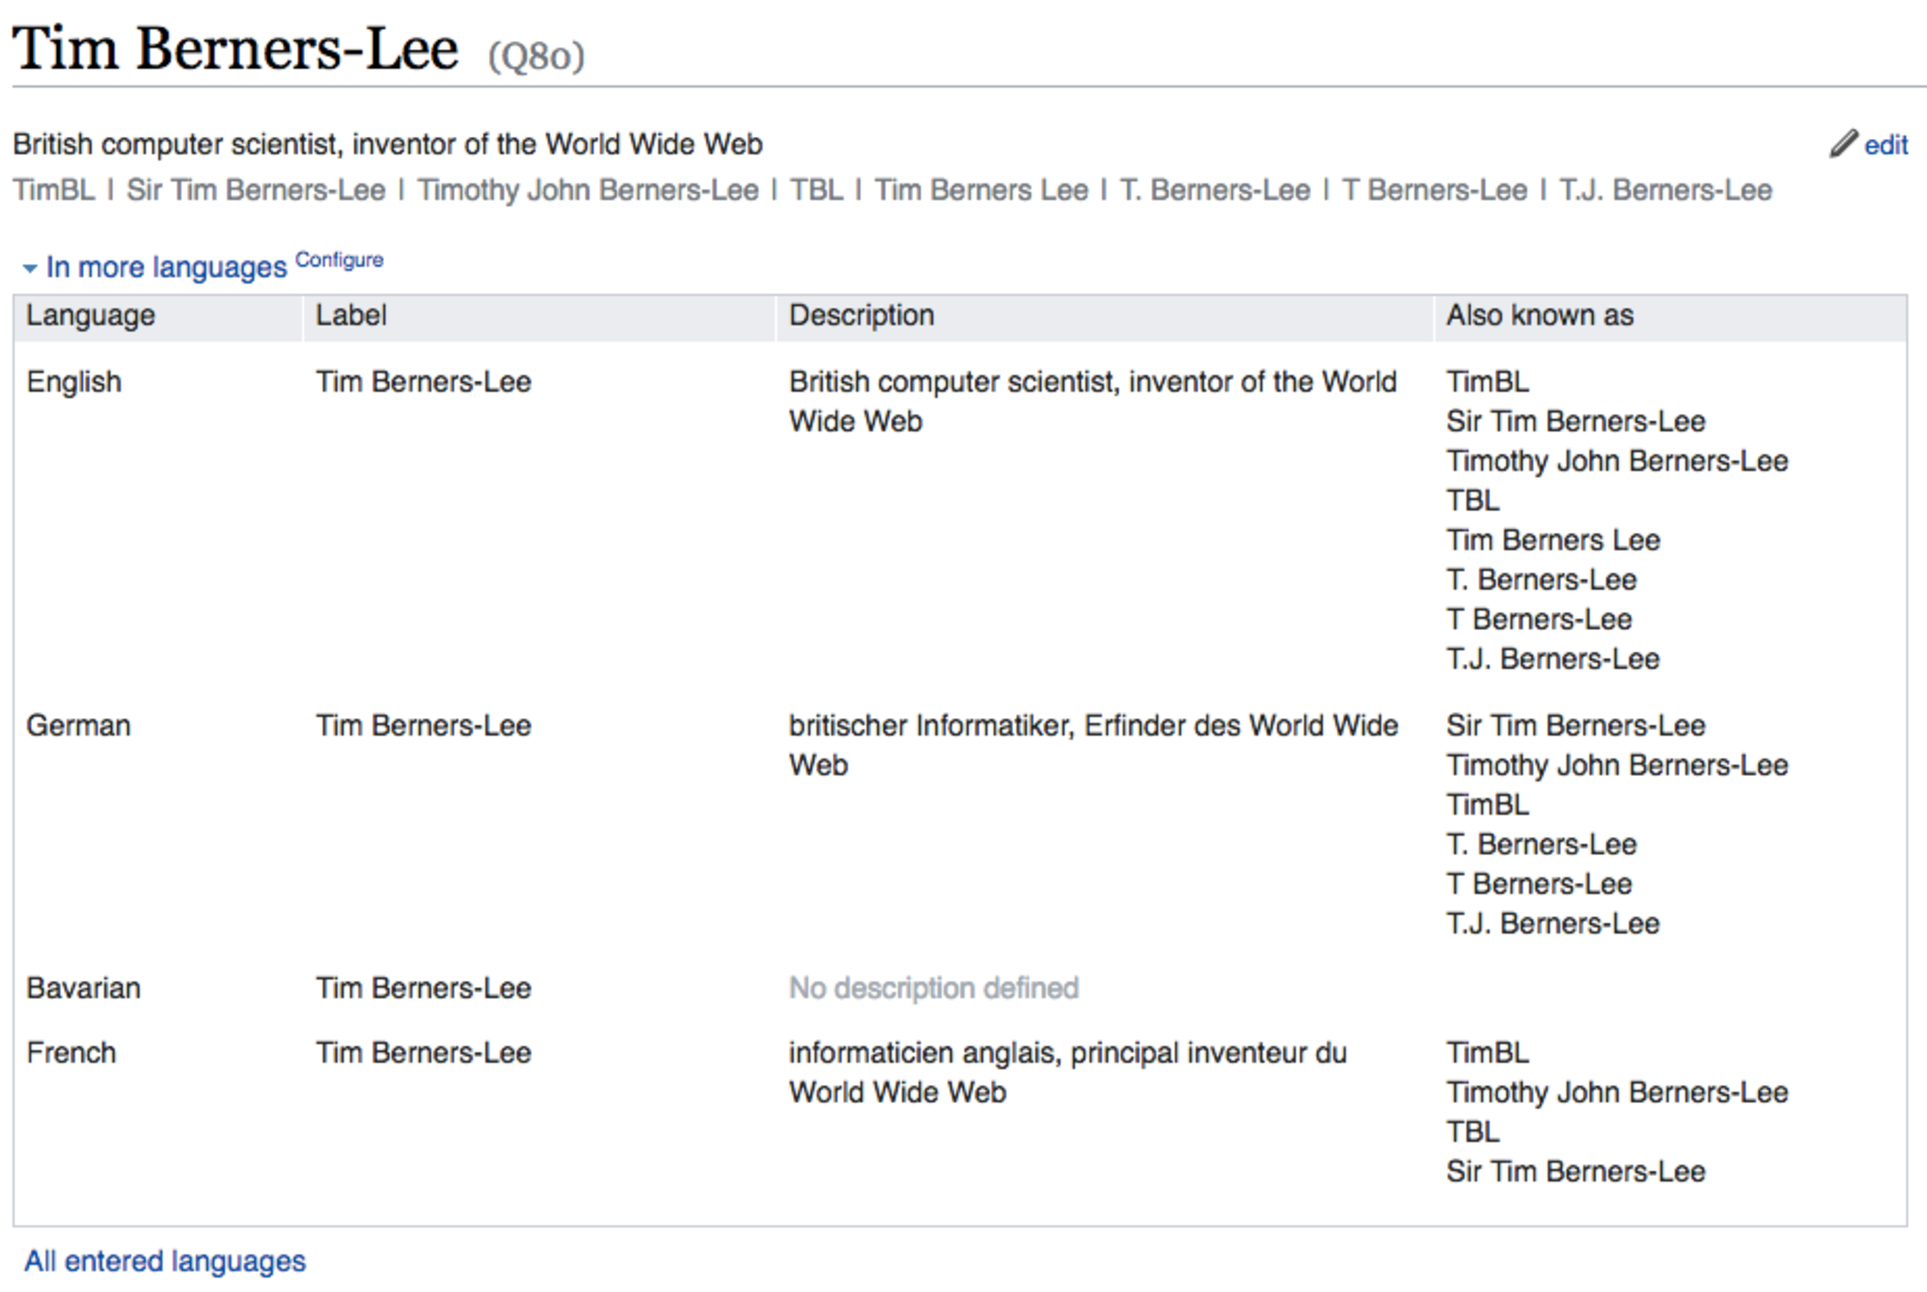
\includegraphics[width=0.75\textwidth]{graphics/wikidata_tim_berners_lee_lang}
	 \caption{Excerpt of a Wikidata page showing language properties of Tim~Berners-Lee}\label{fig:wikidata_tim_berners_lee_lang}
\end{figure}
\begin{figure}
	 \centering
	 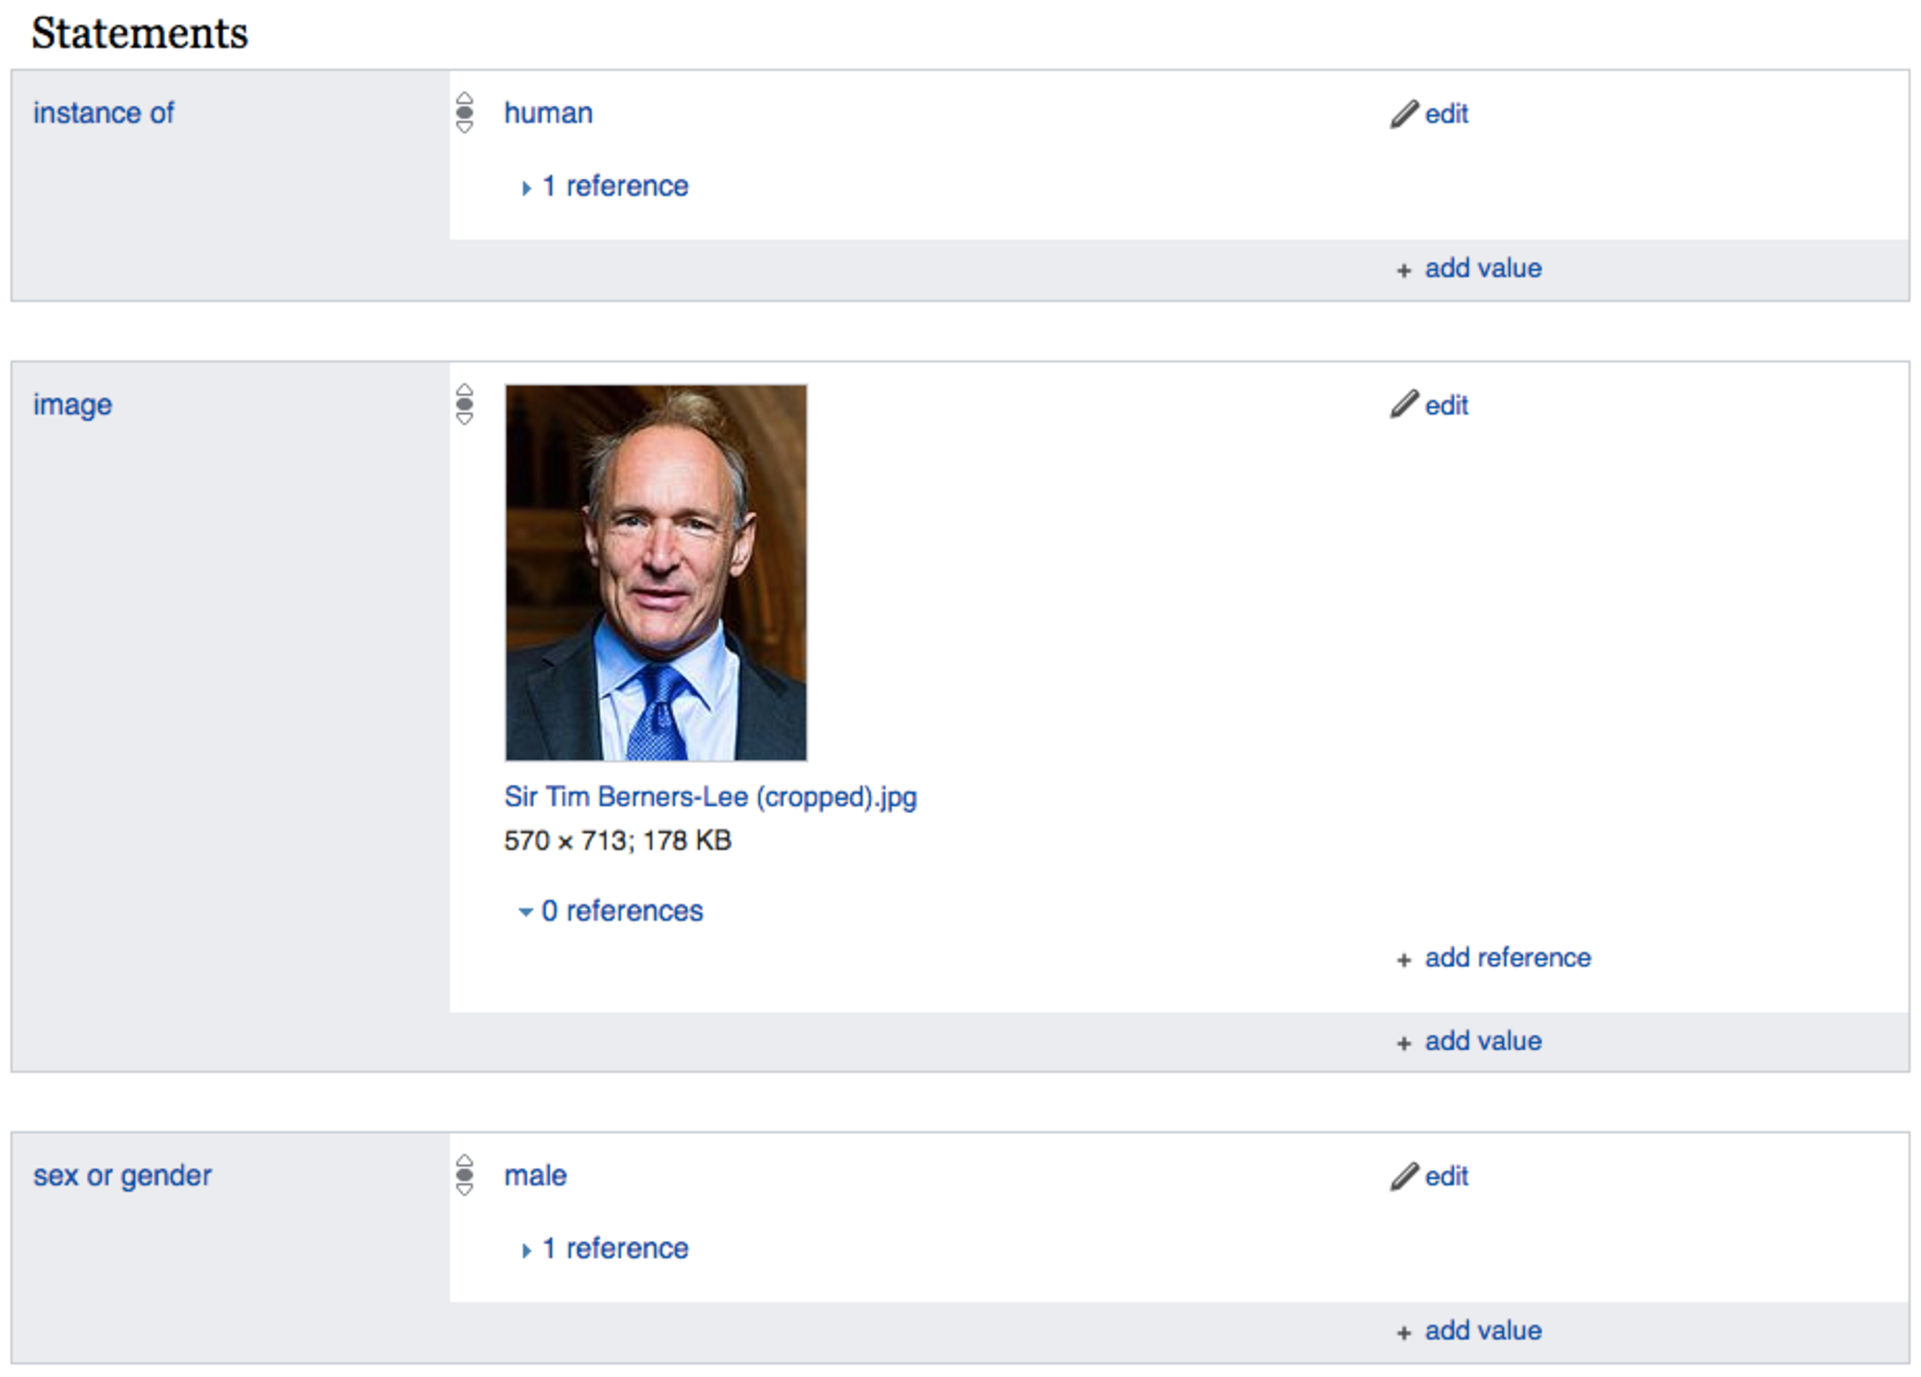
\includegraphics[width=0.75\textwidth]{graphics/wikidata_tim_berners_lee_stat}
	 \caption{Excerpt of a Wikidata page showing statements of Tim~Berners-Lee}\label{fig:wikidata_tim_berners_lee_stat}
\end{figure}
Every page has a unique identifier~(e.g. \texttt{Q80}), a label~(e.g. \texttt{Tim~Berners-Lee}), a brief description~(e.g. \texttt{British computer scientist, inventor of the \gls{www}}), a list of aliases~(e.g. \texttt{TimBLSir, Tim Berners-LeeTimothy, John Berners-Lee, \ldots}), a list of statements~(e.g. \texttt{instanceof, image, \ldots}) and some links. 
It is obvious that these data would perfectly fit into the Linked Data model~\cite{erxleben2014}.
Wikidata content is also available in \gls{rdf} which is accessible at \url{http://tools.wmflabs.org/wikidata-exports/rdf/}. Unfortunately, this data is provided via dump files\footnote{\url{https://tools.wmflabs.org/wikidata-exports/rdf/exports.html} accessed 2018/08/06} only.

\paragraph{Data Storage and Indexing} 
Up to this stage, the data was already mapped to the \gls{rdf} data model but needs to be stored and indexed efficiently. Researchers have put a lot of effort into this field because efficient storage and indexing mechanisms are fundamental for the adoption of Linked Data. Due to efficient querying and storage capabilities of relational databases resulting from decades of research in this area, it makes sense to adopt these approaches for Linked Data as well~\cite{abadi2007}. However, to support storing very large quantities of data there exist custom solutions too~\cite{broekstra2002}. Targeting Linked Data indexing, various approaches and principles have been applied successfully. The common aspects of all approaches is their focus on \emph{Data Compression} and \emph{Data Pruning}~\cite{svoboda2011}. Whereas the basic idea of Data Compression is to minimise the footprint of the index, Data Pruning is a technique for avoiding unnecessary data processing. 

Whereas Data Indexing is traditionally done solely by machines, there are some approaches that combine Crowdsourcing and Semantic principles for Data Storage. One of them is the \gls{led}\footnote{\url{https://led.kmi.open.ac.uk/} accessed 2019/04/01}, a semantic knowledge base of accounts of listening to music in documented sources~\cite{adamou2014}. \gls{led} stores listening evidences of music across history and musical genres. Its dataset includes more than \numprint{10000} entries collected from various sources, volunteers from the crowd being one of them. 

\paragraph{Data Revision and Authoring} In this stage users are given the opportunity to create new or modify existing semantic information. 
This is called \textit{\gls{sca}} which is defined in the literature as~\textit{"a tool-supported
manual composition process aiming at the creation of semantic documents."}~\cite{khalili2013} More generally speaking, \gls{sca} is actually embedded in a broader ecosystem for semantic content authoring as shown in~\hyperref[fig:authoring_semantic_ecosystem]{Figure~\ref*{fig:authoring_semantic_ecosystem}}. 
\begin{figure}
	 \centering
	 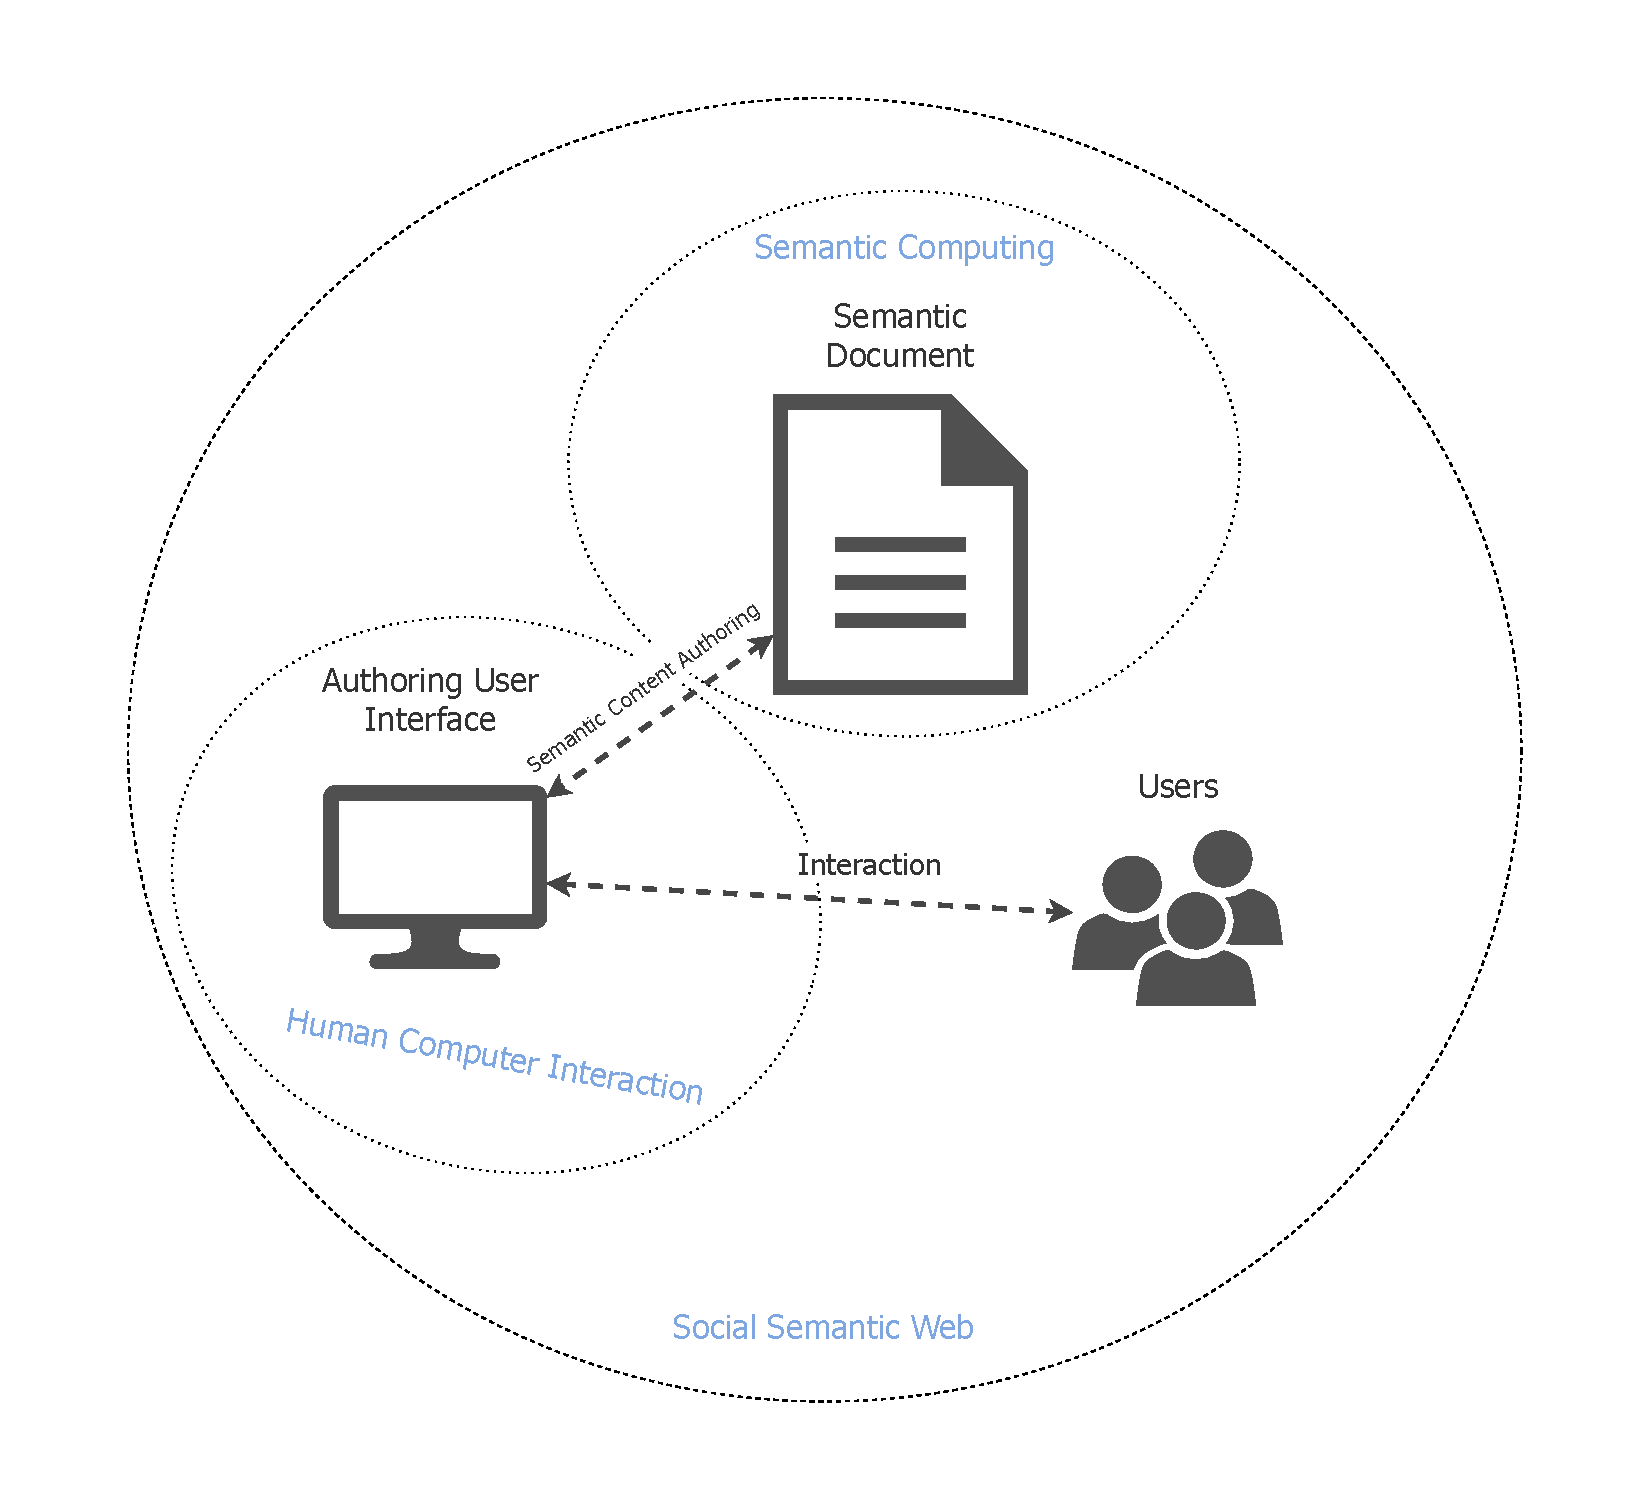
\includegraphics[width=1\textwidth]{drawio/authoring_semantic_ecosystem}
	 \caption{The ecosystem for semantic content authoring}\label{fig:authoring_semantic_ecosystem}
\end{figure}
The central entity of the semantic ecosystem is a semantic document which holds semantically enriched information. 
In information management, semantic documents serve a number of purposes such as information searching, information retrieval, information presentation, information integration, personalisation, reusability and interoperability~\cite{khalili2013}. For that reason there exists a research area dealing with the main fields of semantic content management. In particular, it covers the manipulation, creation and processing of semantic content. Users do not directly interact with semantic documents, but rather through a uniform \gls{ui}. A number of quality attributes for the assessment of \gls{ui}-features of \gls{sca}-Systems were proposed~\cite{khalili2013}. The goal was to improve usability, a measure of the effectiveness, efficiency and satisfaction a user achieves. 

A number of tools for semantic content authoring were developed. A prominent example is OntoWiki~\cite{auer2006}, an open-source Semantic Wiki originally focusing on collaboration but evolved as an ontology editor and platform for knowledge acquisition. It was inspired by other Wiki systems but primarily focusing on managing \gls{rdf} knowledge bases.  Another tool, adding Crowdsourcing capabilities to ontology development activities is Mechanical~Protege\footnote{\url{http://people.aifb.kit.edu/yt2652/mechanicalProtege/}}. The tool is actually a plug-in for the ontology editor Protege\footnote{\url{https://protege.stanford.edu/} accessed 2018/08/07}. 

\paragraph{Data Linking}
The next principle according to the Linked Data Life-Cycle is the Data Linking principle. It is by far the most important principle because it 
underlines the distributed nature of Linked Data. Instead of the traditional definition of data where information is stored in silos with little or no 
relations to the outside, Linked Data sources are distributed, containing many links to other data sources. This paradigm perfectly fits into the distributed nature of the Web, turning it into a source of distributed information optimised for querying and browsing. 

\paragraph{Classification and Enrichment}
Over time, Linked Data sources grow in size and expressiveness. This principle refers to the process of extending the expressiveness and richness 
of semantic knowledge bases. It means that instead of creating the structure upfront, the knowledge base evolves over time. For that, the knowledge 
base is typically enriched by analysing existing data to improve or extend its schema. A variety of (semi-)~automatic enrichment approaches emerged over the past years. The methods span across several research areas, including machine learning, statistics, natural language processing, to name just a few. 

\paragraph{Data Analysis and Quality}
Due to the distributed nature of Linked Data where information originating from heterogeneous data sources is merged, the quality of the resulting
dataset is often varying. Therefore, a key factor for the adoption of Linked Data is ensuring its quality by identifying and fixing common problems. Before that, it is necessary to determine the quality of the existing dataset. For that, metrics which measure the quality in terms of accuracy, completeness, adequacy and degree of understandability need to be defined. \cite{zaveri2016} defines useful quality metrics along with 26 quality dimensions that help to measure the quality of the Linked Data.

\paragraph{Data Cleansing and Evolution}
After the quality is analysed and problems are detected, strategies for fixing these problems are needed. In constantly evolving datasets with millions or even billions of \gls{rdf} triples it is important to keep the links between datasets. Likewise, conflicts and discrepancies in datasets can cause real trouble. Repairing such inconsistencies in overlapping datasets is called \emph{Data Fusion}. Several works focusing on repairing problematic datasets appeared in the literature. For example, \cite{mendes2012} considers repairing with respect to data fusion and \cite{flouris2012} investigates how provenance helps to improve the quality of Linked Data. In this context, provenance refers to where and how the data was obtained from. 

\paragraph{Data Browsing and Querying}
Last, users have the opportunity to explore the Linked Data available on the Web in a fast and efficient way. A prominent way to query Linked Data is
\gls{sparql}\footnote{\url{https://www.w3.org/TR/rdf-sparql-query/} accessed 2019/01/17}, a query language specifically designed to retrieve and manipulate Linked Data. There are similarities between \gls{sql} and \gls{sparql} in terms of query structure, but there are also differences.

LexiTags~\cite{veres2013} is an example which combines Semantic Browsing and Crowdsourcing. It was initially designed as a tool for content management and emerged to a platform that expose crowdsourced semantic metadata to clients, both for creation and consumption of metadata. Its main interface keeps a list of bookmarked URLs, allowing users to add and edit semantic tags. Semantic tagging is a very powerful innovation which helps users to navigate through large datasets by constructing search queries from a set of semantic tags. 



% SECTION: THE UCOMP PLUGIN %
\newacronym{owl}{OWL}{Web Ontology Language}

\section{The uComp Protege Plugin}\label{sec:ucomp_protege_plugin}
In this section we present the uComp Protege Plugin~\cite{wohlgenannt2016} on which our implementation builds on. The plugin was realised as a plugin for the Protege~ontology~editor\footnote{\url{https://protege.stanford.edu/} accessed 2018/08/07}. It enables the automatic creation of Crowdsourcing tasks to support ontology validation, especially as part of Stage 6 and Stage 7 of the Linked Data Life-Cycle in~\hyperref[sec:ld_lifecycle]{Section~\ref*{sec:ld_lifecycle}}. It was designed as a tool used by ontology engineers to reduce the burden of manual ontology validation.

\subsection{Plugin Functionality}\label{sec:ucomp_protege_plugin_functionality}
The plugin supports the following tasks which were previously performed by ontology experts in collaboration with domain experts:

\paragraph{Verification of Domain Relevance}
The goal of this task is to decide whether a given concept~(or a set of concepts) is relevant for a given domain. For that, crowd workers need to
answer a binary question, that is a question with a yes/no answer. The corresponding Crowdsourcing task is automatically generated by the platform and
contains besides the actual concept that should be validated also the domain and optionally some additional information that is useful for answering 
the question. 

\paragraph{Verification of Relation Correctness}
Judging the correctness of relations, the plugin offers interfaces that allow the validation of subsumption and instanceOf relations. 
For subsumption, the crowd needs to decide whether a given concept is a subclass of another concept. For example, validating the correctness
of the subclass relation \emph{isSubClass(weather, rain)} for the domain \emph{climate change}, crowd workers have to decide whether the concept rain is a sub-class~(sub-concept) of the concept weather in the domain of climate change. For validating the correctness of instanceOf relations, the crowd needs to decide whether a given individual is an instance of a given concept~(class). For example, contributors where asked to decide whether the individual \emph{Bordeaux Region} is an instance of the concept \emph{Region} for the \emph{Wine} domain. 

\paragraph{Specification of Relation Type}
This task is different from the others described above. Instead of answering binary questions, the crowd is asked to assign relation types to unlabeled object properties. A prerequisite for this task is that object properties that are selected for evaluation were previously labelled as \emph{relation}. This way, the plugin knows which object properties take part in the validation process. Additionally, crowd workers can optionally suggest a new relation type if none of the suggested ones fit their needs. 

\paragraph{Verification of Domain and Range}
The purpose of this task is mainly to identify problems that are relevant for reasoning rather than validating the ontology structure itself. In this task, the crowd was asked to validate domain and range restrictions as specified by \gls{owl}. For example, the crowd needs to decide whether the object property \emph{hasSister} maps a person~(domain) to a female~(range). As stated earlier, errors in range and domain restrictions have no impact on the ontology itself but are rather used by reasoners to infer additional knowledge. 

\subsection{Validation Workflow}
Supporting ontology engineers was a major design goal of the uComp Protege Plugin.
The workflow to create Crowdsourcing tasks that facilitate ontology validation is depicted in~\hyperref[fig:ucomp_protege_plugin_workflow]{Figure~\ref*{fig:ucomp_protege_plugin_workflow}}.
It involves the following steps:
\begin{figure}
	 \centering
	 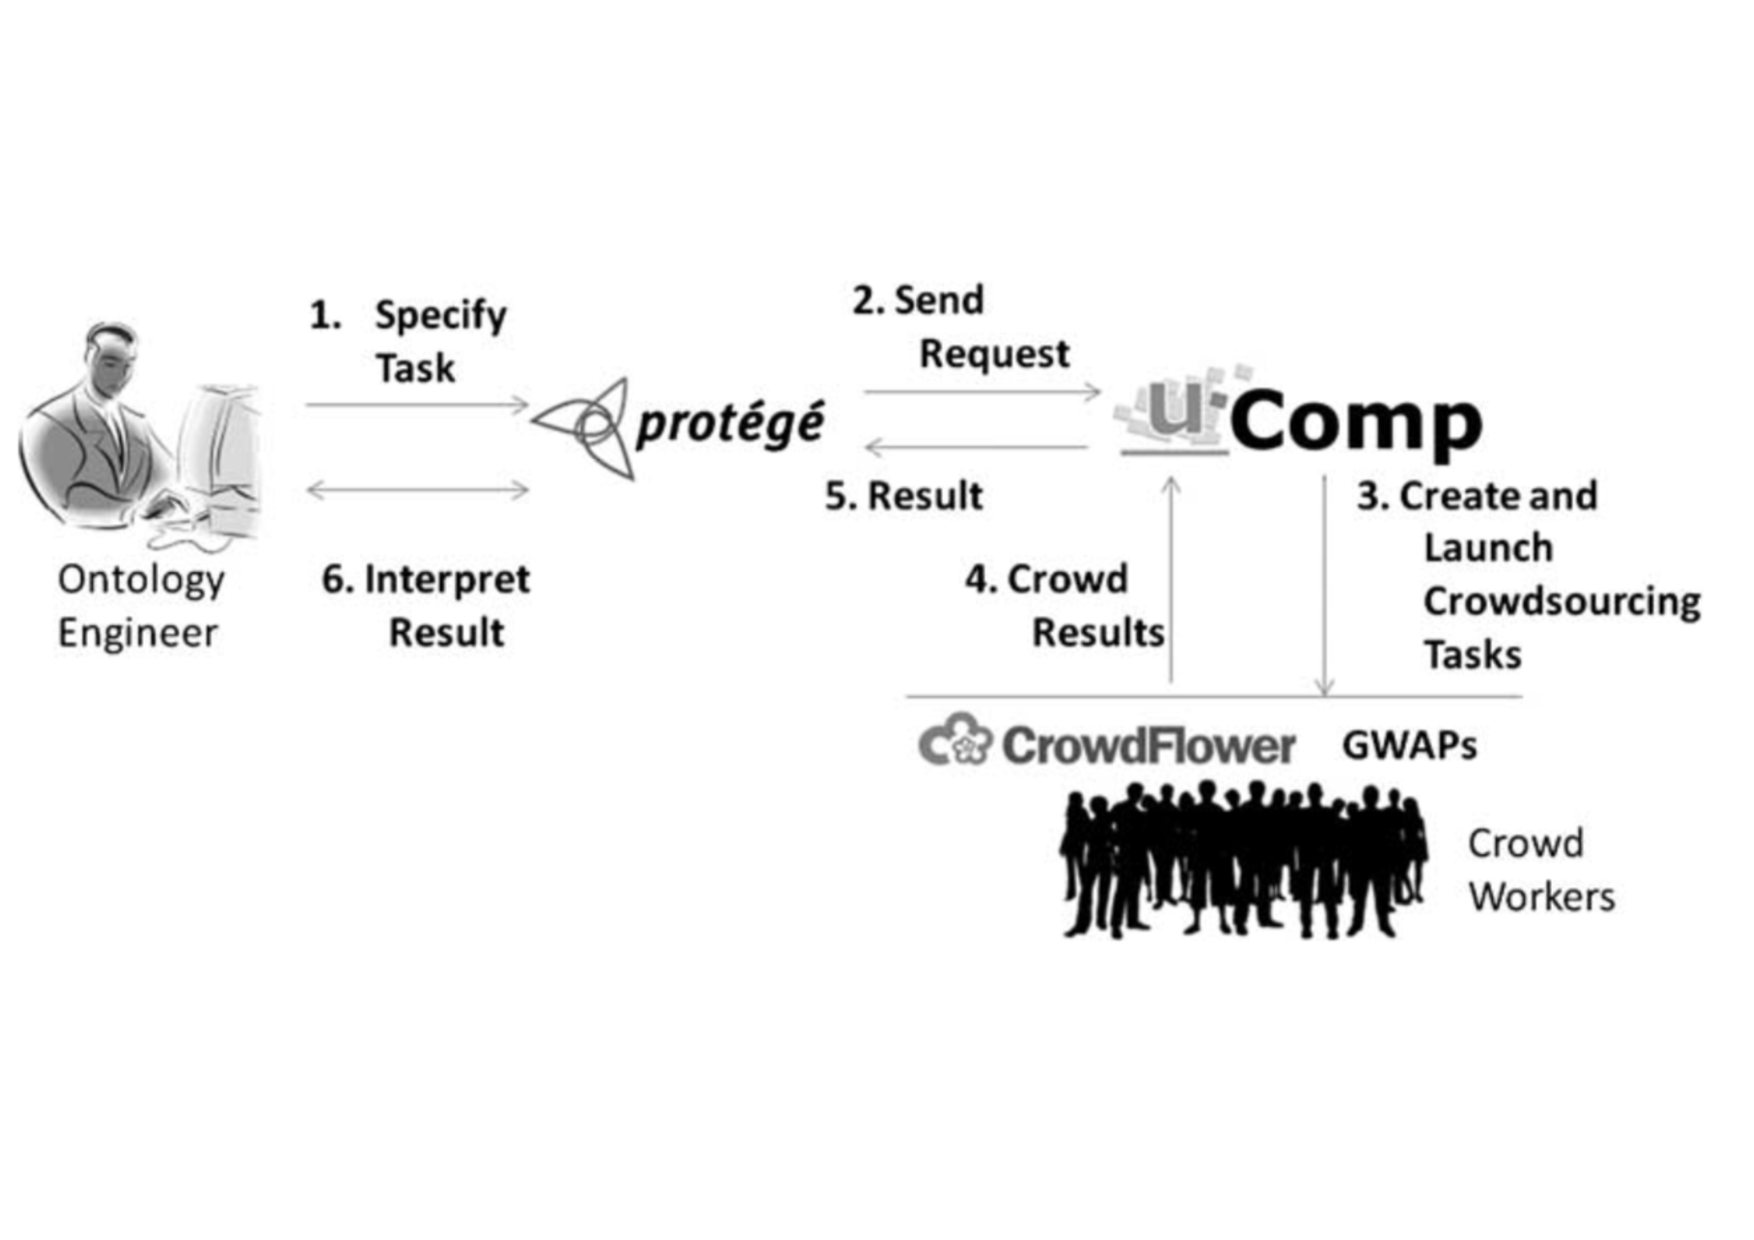
\includegraphics[width=\textwidth]{graphics/ucomp_protege_workflow}
	 \caption{Main workflow to create Crowdsourcing tasks by the uComp Protege Plugin~(adopted from~\cite{wohlgenannt2016})}
	 \label{fig:ucomp_protege_plugin_workflow}
\end{figure}

\begin{enumerate}[label=\textbf{Step \arabic*},leftmargin=\widthof{Step 1}+\labelsep]
	\item \emph{(Task Specification)} In the beginning, the ontology engineer needs to choose from the tasks listed
	in~\hyperref[sec:ucomp_protege_plugin_functionality]{Section~\ref*{sec:ucomp_protege_plugin_functionality}}. For each
	task a standalone interface was created which allows controlling task specific behaviour. 
	\item \emph{(Request Sending)} Next, the plugin gathers the information required to send a request to the uComp platform.
	Unfortunately, at the time of writing this thesis the platform is no longer maintained which required us to directly send the request to the Crowdsourcing provider.  
	\item \emph{(Crowdsourcing Job Creation)} The uComp platform then collects all the data required to create the Crowdsourcing job for the selected Crowdsourcing provider. Initially, the uComp platform supported Crowdflower~(which is now Figure~Eight\footnote{\url{https://www.figure-eight.com/} accessed 2018/07/16}) as the only Crowdsourcing provider. However, the creators of the uComp platform added the option to support other providers as well. 
	\item \emph{(Fetching Crowdsourcing Results)} After job completion~(possibly lasting for several days), the results from the selected Crowdsourcing provider were collected.
	\item \emph{(Aggregating Crowdsourcing Results)} The uComp platform collects all the results~(possibly originating from different platforms) and 
	then calculates the combined result.
	\item \emph{(Result Interpretation)} The last step in the validation workflow is presenting the results to the ontology engineer. Depending on the chosen validation task, further actions may be taken. For example, in case the majority declined the relevance of a specific concept, the ontology engineer may decide to delete the corresponding concept. For all ontology manipulations, the plugin requires manual intervention.
	One of the design goals of the plugin was the guide ontology engineers in doing specific maintenance tasks rather than replacing them by performing these actions automatically. 
\end{enumerate}


% SECTION: CONTEXT ENRICHMENT OF CROWDSOURCING TASKS %
\section{The use of Context in Crowdsourcing Tasks}\label{sec:the_use_of_context_in_crowdsourcing}
% Notes from meeting with MS:
% 
% -) In related work, consider the use of context (e.g. define what "Context" means --> see definition from MS)
% -) Use table with references provided by MS

\subsection{Context}\label{sec:context_in_crowdsourcing_tasks_context}
When analysing the use of Context in crowdsourcing tasks, we noticed that there exists no formal definition of the term \guillemotright Context\guillemotleft~. In fact, all approaches that were found use a different notion of that term. 
This section first investigates what context definitions these approaches use. After that, we give a consolidated definition that fits our approach of crowd-based ontology validation.

When investigating the use of Context in crowdsourcing tasks, a good start is to look at~\cite{sarasua2015crowdsourcing}. In this work, the authors did an extensive literature study to find challenges in the context of Crowdsourcing and the Semantic Web. One of the challenges they found was a proper definition of Context as part of a complete task design. Concretely, they asked but did not answer the minimum required context a crowd needs to finish a task correctly. Unfortunately, during our studies we could not find an answer either. It seems that there exists no generic answer which applies in all contexts, it rather depends on the concrete type of task that needs to be solved. 

During our literature research we found that approaches can be categorised as tasks supplying \textbf{explicit Context}, tasks supplying \textbf{implicit Context} and those providing \textbf{no Context} at all. 

The most obvious work supplying \emph{no~Context} with crowdsourcing tasks was actually done by~\cite{wohlgenannt2016}. It represents the baseline of our work and motives our use of Context. A detailed explanation of this paper is out of scope for this section. However, a detailed explanation was already done in~\hyperref[sec:ucomp_protege_plugin]{Section~\ref*{sec:ucomp_protege_plugin}}. In another paper, a method of collaborative ontology construction was proposed~\cite{zhitomirsky2017}. The actual definition of the ontology was implemented by a hybrid approach containing the definition of RDF-triples by non-experts~(e.g. students) and their classification by the crowd.

Clearly, the omission of Context does not need to be problematic. Whereas crowd-based ontology validation without Context clearly has its drawbacks, it would not be beneficial if the crowd had additional information in the ontology construction example because the entities that formed the statements that were judged were simple and easy understandable by the crowd. 

The other group of tasks that provide additional information are those tasks supplying \emph{explicit~Context}. Similarly to our approach the authors of \cite{mortensen2015} and \cite{mortensen2016} supplied concept descriptions to improve the quality of the judgements. Their goal was to find inconsistencies and errors in SNOMED~CT, a widely used ontology mainly used in biomedical contexts. Even though biomedical ontologies are well documented, not all entities have definitions. For that, English language definitions were manually added by domain experts. 

The last category contains tasks with \emph{implicit~Context}, meaning that Context was not intentionally added. Context is rather defined implicitly, e.g. all Context is already present in the initial dataset. Hence, no additional process or algorithm is needed to define contextual information. For example, in~\cite{acosta2018} the authors used a crowdsourcing data quality assessment tool to detect errors in Linked Data. 
For their analysis they used DBPedia~\cite{auer2007} as evaluation source. Because one of the design principles of DBPedia was to derive linked information from Wikipedia\footnote{\url{https://www.wikipedia.org/}}, it seems natural to add the link to the corresponding Wikipedia page to the crowdsourcing task interface. To that end, no additional process or method for the enrichment of Context exists because the evaluated dataset already contains the Context.

A different approach was taken by~\cite{sabou2018, winkler2017, winkler2017_2} in which an Extended Entity Relationship~(EER)~diagram was verified against a software specification document in a software engineering use case. The diagram, initially created by students, was presented together with the specification text to detect and correct inconsistencies in the conceptual model. From the task description it seems obvious that no additional information is needed because Context was already given implicitly by the EER~diagram. In that sense, the Context was defined in terms the specific task that was carried out by the crowd. 

Taken together all insights from above, we define \guillemotright Context\guillemotleft~in crowdsourcing tasks as:

\begin{defn}
	\emph{(Context)} Context refers to any sort of additional information that is supplied with a crowdsourcing task to improve its understanding in
	such a way that it positively affects the crowds performance and the result quality. Furthermore, we do not set a limitation on the type or format 
	of Context that is provided. Examples are natural language descriptions, links to external content or pictures. We distinguish between
	crowdsourcing tasks that
	\begin{inparaenum}[1)]
			\item supply explicit Context,
			\item those that supply Context implicitly and
			\item those that provide no Context at all.
	\end{inparaenum}
\end{defn}

\subsection{Approaches that Context in Crowdsourcing Tasks}
Based on the definition of \guillemotright Context\guillemotleft~in~~\hyperref[sec:context_in_crowdsourcing_tasks_context]{Section~\ref*{sec:context_in_crowdsourcing_tasks_context}}, in this section we give an overview of various approaches that use~(or omit) Context in crowdsourcing tasks.
\hyperref[table:approaches_of_context_in_crowdsouring_tasks]{Table~\ref*{table:approaches_of_context_in_crowdsouring_tasks}} summarises all approaches that were discussed in this section.

\begingroup
\renewcommand{\arraystretch}{2.5}
\begin{table}
	\begin{tabularx}{\textwidth}{X l*{4}{Y}}
		\toprule
		Paper & Evaluated Unit & Evaluation Target & Context Type & Context \\
		\midrule
		\cite{acosta2018} & RDF triples & Data Quality & Implicit Context & Wikipedia Link \\
		\cite{mortensen2015, mortensen2016} & Ontology Structure & Data Quality & Explicit Context & Concept Descriptions \\
		\cite{sabou2018, winkler2017, winkler2017_2} & Conceptual Model & Data Quality & Implicit Context & EER Diagram \\	
		\cite{wohlgenannt2016} & Ontology Structure & Data Quality & No Context & No Context \\			
		\cite{zhitomirsky2017} & RDF triples & Data Definition & No Context & No Context \\
		\bottomrule
	\end{tabularx}
	\caption{Overview of approaches that Context in crowdsourcing tasks}
	\label{table:approaches_of_context_in_crowdsouring_tasks}
\end{table}
\endgroup

The first approach~\cite{acosta2018} investigates quality issues along the two dimensions accuracy and interlinking. The attributes that were evaluated by the crowd were incorrect object values, incorrect datatypes or language values and incorrect links. The evaluation was performed on a linked dataset extracted from the DBPedia corpus. The quality assessment consisted of a twofold approach. In the first stage, a group of Linked Data experts had to select possible candidates of RDF-triples that might have quality problems. In the second stage, the triples were evaluated by the crowd. Because DBPedia triples were constructed by knowledge extraction from Wikipedia, it seemed appropriate to display the link to the corresponding Wikipedia page which served as context. Even though the results were promising, the full potential could possibly be reached by a hybrid approach which combines crowd-based evaluation with an automatic process that helps to reduce the number of triples that resort to crowdsourcing. 

The next work was initially proposed by~\cite{mortensen2015} and then extended by~\cite{mortensen2016} to verify the quality of hierarchical relations in biomedical ontologies. They selected a random subset of 200 subsumption relations from SNOMED~CT, an ontology that often serves as knowledge source in biomedical contexts. For the evaluation, the crowdsourcing task was generated from subsumption relations and concept descriptions. Due to the complexity of the application domain, biomedical ontologies are well documented and naturally contain many concept descriptions. Those concepts with missing descriptions were enriched with documental information. The authors concluded that crowdsourcing can compete with manual evaluation done by medical experts, however, certain tasks, especially more complex ones that are poorly documented, should be better done by domain experts. 

A couple of researchers~\cite{sabou2018, winkler2017, winkler2017_2} investigated conceptual model verification from a Software Engineering perspective. They used crowdsourcing techniques to verify the correctness of Extended Entity Relationship~(EER)~diagrams. In their first experiment, students had to create the conceptual model~(EER-diagram) from a specification document which was written in informal English language. The resulting models~(diagrams) were then checked by the crowd to identify inconsistencies between the model and the specification text. In this setting, the EER-diagram served as Context for the crowdsourcing task. Their experiments achieved high precision and recall, however a few shortcomings will be addressed in their future work. 

While all the crowdsourcing tasks discussed so far had contextual information to some extend, the approaches presented next completely omit Context. 
For example,~\cite{wohlgenannt2016} represents the baseline of our work and motives our use of Context. A detailed explanation was already done in~\hyperref[sec:ucomp_protege_plugin]{Section~\ref*{sec:ucomp_protege_plugin}}.

The last paper that is discussed in this section is~\cite{zhitomirsky2017}. It covers the process of ontology construction, a costly and time consuming task that involves extensive expert participation. In this work, the authors presented a two-step approach. It consists of collaborative ontology construction by non-experts and classification of statements that were formed from RDF-triples. Special attention was paid towards the reduction or omission of subjective or biased judgements. For that, multiple viewpoints were merged to create a unified multi-viewpoint ontology.
Whereas the initial task of collecting controversial subjects and creating multiple single-viewpoint ontologies was done manually by non-professionals, their classification to form one unified multi-viewpoint ontology was performed by the crowd. 
The results showed that no additional Context is needed if the domain not too complex and the statements~(relations) were easily understandable.  




%%%%%%%%%%%%%%%%%%%%%%%%%%%%%%%%%%%%%%%%%%%%%%%%%%%%%%%%%%%%%%%%%%%%%%%%%%%%%%%%%%%%%%%%%%%%%%%%%%%%%%%%%%%%%%%%%%%%%%%%%%%%%%%%%%%%%%%%%%%%%%%%%%%%
